\documentclass[12pt]{article}
%\usepackage{natbib}
\usepackage[spanish]{babel}
\usepackage{url}
\usepackage[utf8]{inputenc} 
\usepackage{amsmath}
\usepackage{graphicx}
\graphicspath{ {./images/} }
\addto\captionsspanish{\renewcommand{\tablename}{Tabla}}					% Cambiar nombre a tablas
\addto\captionsspanish{\renewcommand{\listtablename}{Índice de tablas}}		% Cambiar nombre a lista de tablas
\usepackage{parskip}
\usepackage{fancyhdr}
\usepackage{vmargin}
\providecommand{\abs}[1]{\lvert#1\rvert}
\providecommand{\norm}[1]{\lVert#1\rVert}
\usepackage{float}
\usepackage{verbatim} 
\usepackage{multirow}
\usepackage{longtable}
\usepackage{biblatex} %Imports biblatex package
\addbibresource{biblist.bib} %Import the bibliography file
\usepackage[colorlinks=true,urlcolor=blue,linkcolor=black,citecolor=black]{hyperref}     % Para insertar hipervínculos y marcadores
\bibliography{biblist}  % Biliografía

\setmarginsrb{1.5 cm}{2.5 cm}{1.5 cm}{2.5 cm}{1 cm}{1.5 cm}{1 cm}{1.5 cm}

\title {AuVeTA: Autonomous Vehicle for Tracking Aplications\\[1 cm]}				

\makeatletter
\let\thetitle\@title
\let\theauthor\@author
\let\thedate\@date
\makeatother

\pagestyle{fancy}
\fancyhf{}
\lhead{AuVeTA proyect}
\rhead{IE-0117}
\cfoot{\thepage}



%%%%%%%%%%%%%%%%%%%%%%%%%%%%%%%%%%%%%%%%%%%%%%%%%%%%%%%%%%%%%%%%%%%%%%%%%%%%%%%%%%%%%%%%%
\begin{document}

\begin{titlepage}


\centering

\includegraphics[width=4 cm]{imagenes/LOGO}\\[1 cm]

	\centering
    \textsc{\LARGE Universidad de Costa Rica}\\	% University Name
	\textsc{ \Large{Escuela de Ingeniería Eléctrica} \\  \large{IE-0117 \\ Programación bajo plataformas abiertas}}  \\[0.5 cm]
	
	\rule{\linewidth}{0.2 mm} \\[0.4 cm]
	{ \huge \bfseries \thetitle}
	\rule{\linewidth}{0.2 mm} \\[1 cm]
	
    Grupo de trabajo 0:

		 Rodríguez Quintana Esteban\hspace{1.5 cm} B66076     \\
		 Jorge Isaac Fallas Mejía\hspace{1.5 cm} B62562 \\
		 Fabio Villalobos Pacheco   \hspace{1.5 cm} B78346\\[2 cm]

	{ Grupo de clase 3} \\				% Course Code 
	 \normalsize Profesor: Ricardo Román Brenes\\[1 cm]

	
		I 2019
	
    
    
    
    
	
\end{titlepage}

%%%%%%%%%%%%%%%%%%%%%%%%%%%%%%%%%%%%%%%%%%%%%%%%%%%%%%%%%%%%%%%%%%%%%%%%%%%%%%%%
\pagenumbering{roman}

\tableofcontents
\pagebreak
%   \listoffigures
%   \listoftables
\pagebreak

%%%%%%%%%%%%%%%%%%%%%%%%%%%%%%%%%%%%%%%%%%%%%%%%%%%%%%%%%%%%%%%%%%%%%%%%%%%%%%%%%%%%%%%%%
\pagenumbering{arabic}

\newpage


\begin{comment}

\section{Objetivos}
\subsection{Objetivo General}

\begin{itemize}
    \item Diseñar y construir un vehículo seguidor de línea capás de remover obstáculos pequeños.
\end{itemize}


\subsection{Objetivos Específicos}
\begin{itemize}
    \item Integrar conocimientos adquiridos en el de Laboratorio Eléctrico I y cursos previos.
    \item Implementar programación de Arduino para la automatización del vehículo.
    \item Concluir el recorrido del vehículo con la activación de un circuito de control.
\end{itemize}
\end{comment}

\newpage

\section{Reseña del proyecto a implementar}

El proyecto AuVeTA consiste en diseñar y poner en funcionamiento un vehículo que pueda ser utilizado como una base para prototipado de un vehículo que a futuro pueda utilizarse en aplicaciones de seguimiento de linea para algún tipo de aplicación industrial o inclusive evolucionar al mundo del reconocimiento de patrones y la visión por computador para generar una propuesta de vehículos realmente autónomos y con aplicación enfocada a la movilidad humana.

Este proyecto consiste en el desarrollo de un vehículo semi autónomo que, mediante la implementación de microcontroladores, sensores, un módulo de comunicación y programación, pueda cumplir con el objetivo de seguir una línea de color en el suelo y llegar a un punto donde culmine con la ejecución de una tarea determinada. Parte de las funciones que se desean incorporar a este prototipo, además del seguimiento de línea y remoción de obstáculos, son la comunicación del vehículo con un centro de control, desde el cual también se pueda conducir a discreción el mismo, con la finalidad de ser utilizado en otro tipo de aplicaciones mediante sus distintos modos de operación.

El proyecto consta de dos partes principales: hardware y software. El desarrollo e integración de estos dos subsistemas han de ir de la mano, puesto que un error en uno de ellos ha de limitar la acción correcta del otro.

\section{Funcionamiento de Software}

El código se implementará en dos etapas, la primera consiste en una etapa de control y la segunda en una etapa de seguimiento, ambas son completamente independientes la una de la otra.

\begin{itemize}
    \item \textbf{Seguimiento}: La etapa de seguimiento implementa el sensor de línea, la idea es regular el funcionamiento de los motores de acuerdo a la corrección que ha de ser necesario para mantener el vehículo encima de la línea a seguir, y garantizar de esta forma seguimiento del trazo deseado. Toda la implementación de este código se hará programada en el IDE de Arduino puesto que al ser la etapa semi autónoma del proyecto no requiere de ningún comando desde un centro de control para la toma de decisiones. 
    Esta etapa de seguimiento implementa 3 sensores, uno para reconocer la línea a seguir, y dos sensores de obstáculo, uno de ellos encargado de detectar obstáculos frente al vehículo para su remoción, y el otro sensor para reconocer cuando se llega al final del recorrido.
    
    \item \textbf{Control}: La etapa de control se encarga de manejar el funcionamiento de los motores de manera remota mediante un módulo bluetooth, la idea es enviar datos desde un programa en C a través del puerto serial. Dependiendo de qué dato sea enviado, el vehículo llevará a cabo distintos movimientos. El programa en C cuenta con distintas funciones que permiten controlar el puerto serial, al cual se conecta el módulo bluetooth, son tres funciones en total. La primera se encarga de inicializar el puerto serial, una vez inicializado se pueden utilizar las otras dos funciones, una para escribir y la otra para leer datos, de esa forma se establece una comunicación bidireccional. Dichas funciones serán implementadas en una interfaz gráfica que simula un control remoto, la idea es controlar el vehículo con el teclado, y con la interfaz visualizar los movimientos que realiza el vehículo.
\end{itemize}







\section{Funcionamiento de Hardware}

\subsection{Microcontrolador ATmega328}
El ATmega es un microcontrolador de baja potencia CMOS de 8 bits. Mediante la ejecución de instrucciones potentes en un solo ciclo, el microcontrolador permite que el usuario optimice el consumo versus la velocidad de procesos. Este microcontrolador forma parte del Arduino UNO, el cual será la placa de hardware sobre la cual se desarrollará el control del vehículo en sus dos modalidades, seguidor de linea y control mediante bluetooh. 

La estructura del \textit{core} combina un conjunto robusto de instrucciones con 32 registros de trabajo. Estos 32 registros se encuentran directamente conectados a la Unidad
Lógica Aritmética (ALU), permitiendo el acceso independiente de dos registros ejecutados en un solo ciclo de reloj \cite{atmega}. 

\begin{figure}[H]
    \centering
    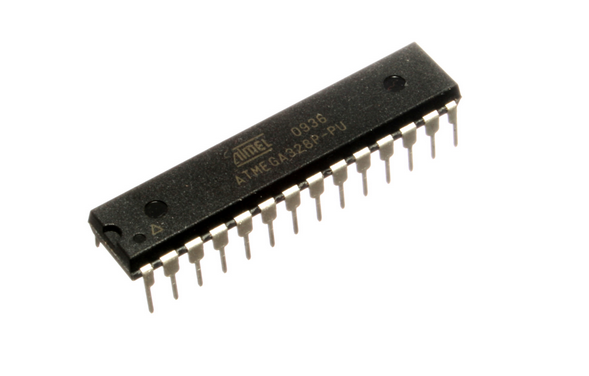
\includegraphics[width = 7 cm]{imagenes/micro.PNG}
    \caption{ATmega 328}
    \cite{atmega}
\end{figure}

\subsection{Sensor de obstáculo}
El sensor de obstáculo opera mediante una configuración emisor-receptor de luz infrarroja. Si la luz infrarroja choca contra un obstáculo, esta será reflejada y detectada por el fotodiodo. El rango de detección puede ser configurado mediante los dos controladores. Si no hay un obstáculo en frente la salida del sensor estará en alto, en el momento que se detecte un obstáculo la señal de salida se apagará.

El sensor permite activar o desactivar la detección de obstáculos mediante la manipulación del pin \textit{enable}. Por defecto, el sensor se encuentra en modo activo \cite{obstaculo}.

\begin{figure}[H]
    \centering
    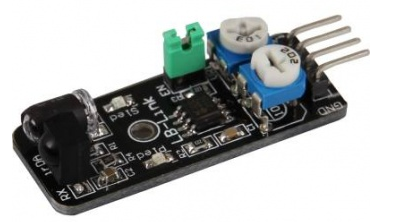
\includegraphics[width = 7 cm]{imagenes/obstacle.PNG}
    \caption{Sensor de obstáculo}
    \cite{obstaculo}
\end{figure}

\subsection{Sensor de traking}
Es un módulo tipo LEGO, listo para ser conectado al microcontrolador. Se basa en un sensor óptico reflexivo con salida de transistor, el cual se encarga de recibir las señales infrarrojas enviadas para detectar la intensidad de la señal. Con cierto rango de altura, los sensores de pista son ampliamente utilizados para vehículos inteligentes o impresoras para detección de líneas en blanco y negro \cite{track}.

\begin{figure}[H]
    \centering
    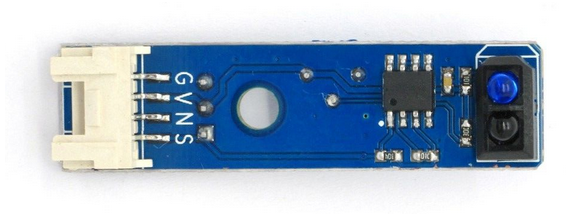
\includegraphics[width = 7 cm]{imagenes/tracking.png}
    \caption{Sensor de pista}
    \cite{track}
\end{figure}


\subsection{Motores DC 200 RPM a escala}
Compuesto por un par de motores DC a escala, son usualmente recomendados como una opción barata y sencilla para poner ruedas en movimiento. Requieren una tensión de 4.5V y una corriente sin carga de 190 mA además posee una caja reductora 48:1 y una velocidad de giro de 200 RPM sin carga \cite{motor_dc}.

\begin{figure}[H]
    \centering
    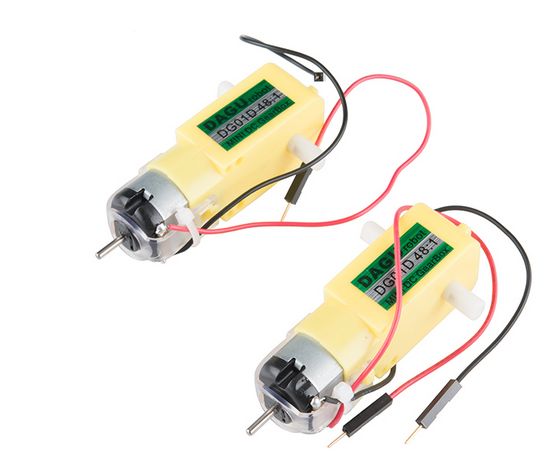
\includegraphics[width = 7 cm]{imagenes/gearmotor.PNG}
    \caption{Hobby Gearmotor - 200 RPM}
    \cite{motor_dc}
\end{figure}

\subsection{Módulo de control de motores DC 800 mA}

El módulo de control L9110S 2-Canales es una tarjeta compacta que puede ser utilizada para controlar robots pequeños. Este módulo posee dos controladores independientes capaces de entregar hasta 800 mA en corriente continua. Pueden operar entre 2.5V y 12V lo cual permite que sean usados mediante microcontroladores.

Mediande control PWM ---\textit{Pulse Width Modulation}--- es posible controlar la velocidad del motor y una salida digital es usada para indicar la dirección \cite{driver}.

\begin{figure}[H]
    \centering
    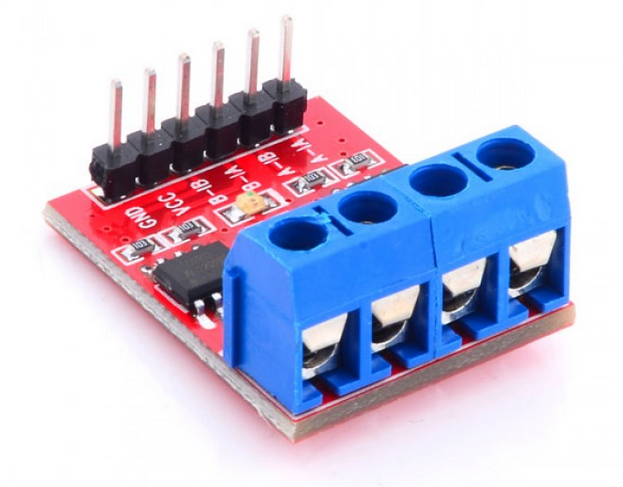
\includegraphics[width = 7 cm]{imagenes/driver.PNG}
    \caption{L9110S Drive Dual Motor DC 800mA}
    \cite{driver}
\end{figure}


\subsection{Servomotor}
El servo es un tipo de motor que funciona paso-a-paso, es decir, su giro se determina en ángulos y no en RPM. Pequeño, liviano y con una alta potencia de salida; este tipo de servomotor es capaz de rotar hasta 180 grados \cite{servo}.

\begin{figure}[H]
    \centering
    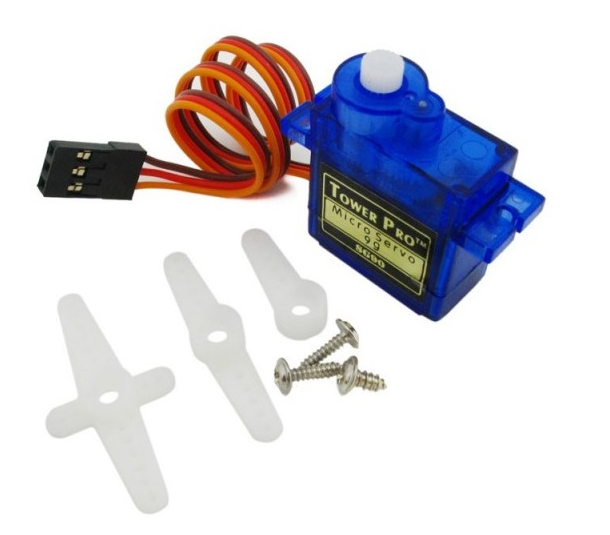
\includegraphics[width = 7 cm]{imagenes/servo.PNG}
    \caption{Servomotor SG90}
    \cite{servo}
\end{figure}

\subsection{Piezo Speaker}
Es un pequeño parlante redondo de 12mm el cual opera en todo el rango audible. Pueden ser utilizados para crear interfaces simples musicales. Requiere de una tensión entre los 3.5V y 5V con una corriente media de 35 mA además de una onda cuadrada para su correcto funcionamiento.

\begin{figure}[H]
    \centering
    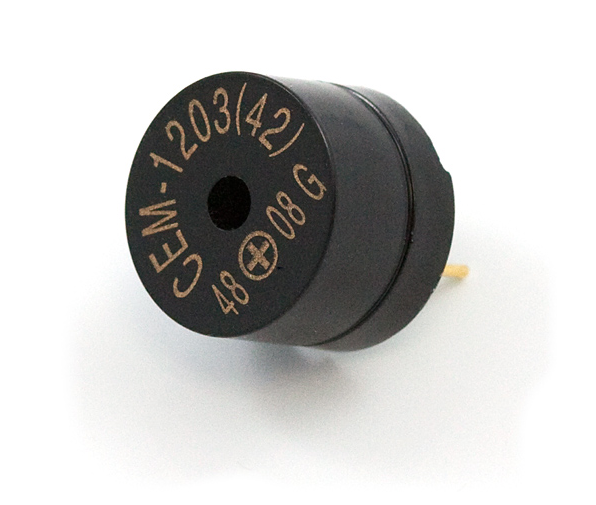
\includegraphics[width = 7 cm]{imagenes/speaker.PNG}
    \caption{Magnetic buzzer}
    \cite{speaker}
\end{figure}

Leer más: \url{https://www.microjpm.com/products/buzzer-timbre-tono-de-alarma-1-5v-3v-6v-12v/}

\subsection{Módulo bluetooth HC-05}
El módulo bluetooth HC-05 se utiliza en este proyecto para poder enviar datos desde un programa en C al arduino, la comunicación se realiza a través del puerto serial, mediante el cual se transmiten los datos. Dichos datos son interpretados por el arduino para llevar a cabo las funciones que el vehículo realiza. 
\begin{figure}[H]
    \centering
    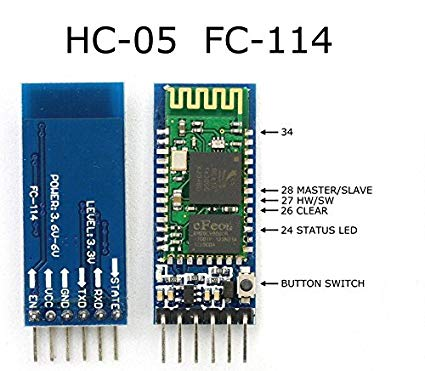
\includegraphics[width= 7 cm]{./imagenes/hc-05.jpg}
    \caption{Módulo bluetooth}
   
\end{figure}


\subsection{Esquemático de conexiones de vehículo}

\begin{figure}[H]
    \centering
    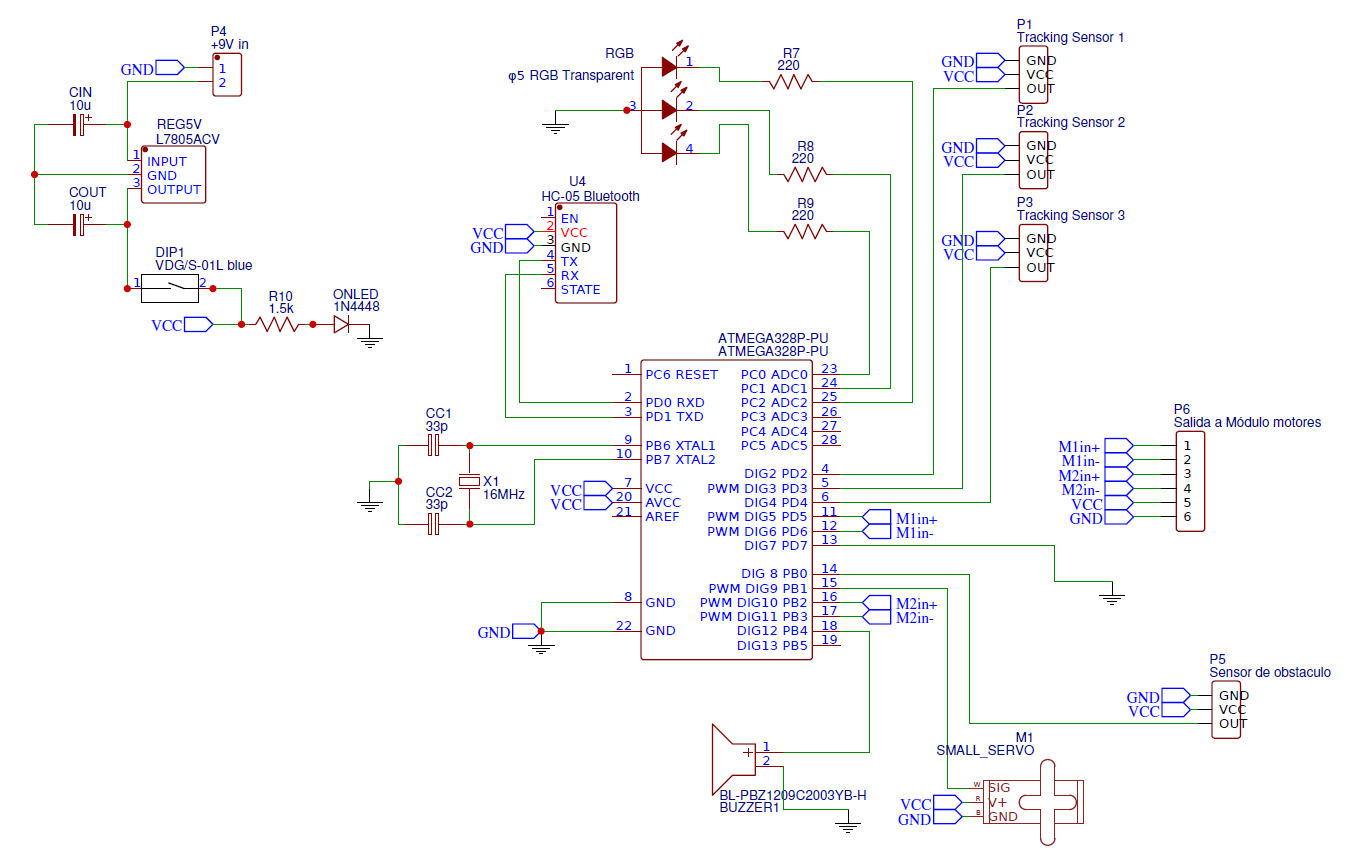
\includegraphics[width = 18 cm]{imagenes/schem_vehiculo.PNG}
    \caption{Esquemático del Vehículo Seguidor de Línea}
\end{figure}


\newpage
\section{Pruebas y validación de programa}

Es importante recalcar que las pruebas son parte fundamental durante el desarrollo y para el éxito de cualquier proyecto, puesto que en esta etapa es donde se puede determinar de manera crítica el funcionamiento de cada uno de los subsistemas que conforman cualquier proyecto. Además, la etapa de pruebas en muchas ocasiones revela posibles puntos de optimización tanto a nivel de software como hardware y en general permite descubrir inconvenientes que puedan existir en la integración e interacciones de dichos subsistemas. 
Este proyecto consta de dos partes estrechamente relacionadas, puesto que el resultado final dependerá tanto del hardware como el software. Cabe resaltar que dentro de las pruebas dividiremos las mismas en:

\begin{itemize}
    \item Pruebas de software.
    \item Pruebas de hardware.
    \item Pruebas de integración.
    \item Pruebas de campo.
\end{itemize}

\subsection{Pruebas de Software}
\begin{itemize}
    \item Revisión de interfaz y posible manejo de errores de comunicación u ocasionados por el usuario.
    \item Asignación correcta de pines en el código de acuerdo al tipo de entrada o salida. 
    \item Verificación de correcta implementación de las bibliotecas en los códigos.
    \item Revisión de cantidad de memoria utilizada por la interfaz y en el arduino.
\end{itemize}

\subsection{Pruebas de Hardware}
\begin{itemize}
    \item Chequeo de continuidad en cables y conexiones.
    \item Verificación de sujeción de componentes en su lugar.
    \item Prueba de cada módulo individualmente para verificar su correcto funcionamiento. 
\end{itemize}

\subsection{Pruebas de integración}
\begin{itemize}
    \item Pruebas con todos los módulos y sensores integrados.
    \item Conexión correcta de pines al Arduino en relación al código.
    \item Cálculo de tiempo de autonomía de fuente de poder con todos los subsistemas en funcionamiento.
\end{itemize}

\subsection{Pruebas de campo}
\begin{itemize}
    \item Control de potencia de las ruedas dependiendo de donde se implemente el vehículo para evitar deslizamiento.
    \item Pruebas de rango de acción de sensores de acuerdo a las condiciones de luz del entorno donde se implemente el vehículo.
\end{itemize}

Todas las pruebas son importantes, pero en el caso de este proyecto se pondrá especial atención a la integración, puesto que la interacción hardware-software puede representar una barrera importante a la hora de implementar los distintos modos de operación del vehículo y su accionar en un entorno físico, por tal motivo, consideramos de esta la prueba más crítica.


\printbibliography

\end{document}